\chapter{Cartes de Kohonen et modèle d'architecture CxSOM}
\graphicspath{{02-SOM/}}
\minitoc
\comment{Idée du chapitre : 

"Qu'est ce qu'on veut faire avec des cartes de Kohonen ?" 
" A quoi servent les cartes de Kohonen ?" ok on les utilise pour de la visualisation, de la réduction de dimension. La visualisation est bien pour un observateur humain, la réduction de dimension peut impliquer qu'on va utiliser un algorithme derrière. Mais les cartes de Kohonen vont plus loin dans l'apprentissage: on a une approximation de l'espace d'entrée par un graphe. Cela veut dire qu'une entrée est associée à un prototype dans la carte, mais inversement : un prototype est associé à un ensemble d'entrée continu ou contigu.
Une entrée est alors représentée par notamment sa position dans la carte : un nombre donc, ou une paire. 
Il est possible de faire du calcul sur ces positions au sein d'algoithmes. 
Dans cette thèse, on a pensé à utiliser cette propriété pour construire un réseau de cartes auto-organisatrices. Par ce réseau, on peut exploiter les positions pour générer des dynamiques au sein de la carte qui permettront une prise de décision, ou des représentation de donnée différentes. 
// Kohonen : il faut surprendre encore ! Par quel 
bout le prendre ? 
→ Appuyer sur les cartes 1D
→ Comment ca se fait qu’on les utilise pas de ouf ? 
→  Intérêt de la topologie de la carte. Dans une carte seule, est ce que c’est vraiment utile ?
→ Questionnement informatique : qu’est ce qui se passe en fait dedans, mais c’est quand même rigolo. }


\section{Carte de Kohonen}

\subsection{Algorithme et notations}

Rappelons les notations concernant une carte de Kohonen standard. Prenons un ensemble de données d'entrées, dans lequel chaque élément est un vecteur d'un espace $D$, dans lequel est définie une distance $d$.
La carte de Kohonon construite sur ces entrées est un graphe, généralement une ligne 1D ou une grille 2D de $N$ noeuds. Chaque noeud possède un poids associé $\w_e in D$ ou \emph{prototype}, du même espace que les entrées. et une \emph{position} $i$ dans la carte. Ces positions sont ensuite indexées entre $0$ et $1$ par $p= \frac{i}{N}$ pour l'homogénéité des calculs. 
L'ensemble des poids est noté ${\w_e(p), p \in [0,1]}$. 
L'algorithme se décompose de la façon suivante :

\begin{enumerate}
\item Une entrée $\inpx_t$ est présentée à la carte.
\item L'unité ayant le poids le plus proche de $\inpx_t$ selon la distance $d$ est choisie comme \emph{Best Matching Unit} de la carte. Sa position est notée $\bmu$.
\item Chaque poids $\w_e$ est déplacé vers l'entrées $\inpx$, en fonction de sa distance dans la carte à la best matching unit : 
\begin{equation}
\w_e(p,t+1) = \w_e(p,t) + \alpha h(\bmu,p)(\inpx - \w_e(p,t))
\label{eq:update}
\end{equation}
\end{enumerate}

$h(\bmu,p)$ est la \emph{fonction de voisinage}. Elle est maximale en $p = \bmu$ et décroissante autour de cette position. Dans notre étude, les fonctions de voisinage sont triangulaires, donc maximales en $\bmu$, décroissante sur le rayon de voisinage $h_e$ et nulle après.

Lors de l'étape 2 de l'algorithme, une activité peut être calculée, au lieu d'une distance pour choisir le BMU. Ce dernier est alors choisi comme $\bmu = \argmax_p (a(\inpx,p)$. Nous utiliserons cette solution dans notre modèle. Les notations au sein d'une carte sont résumées en figure~\ref{fig:one_map_not}.

\begin{figure}
\centering
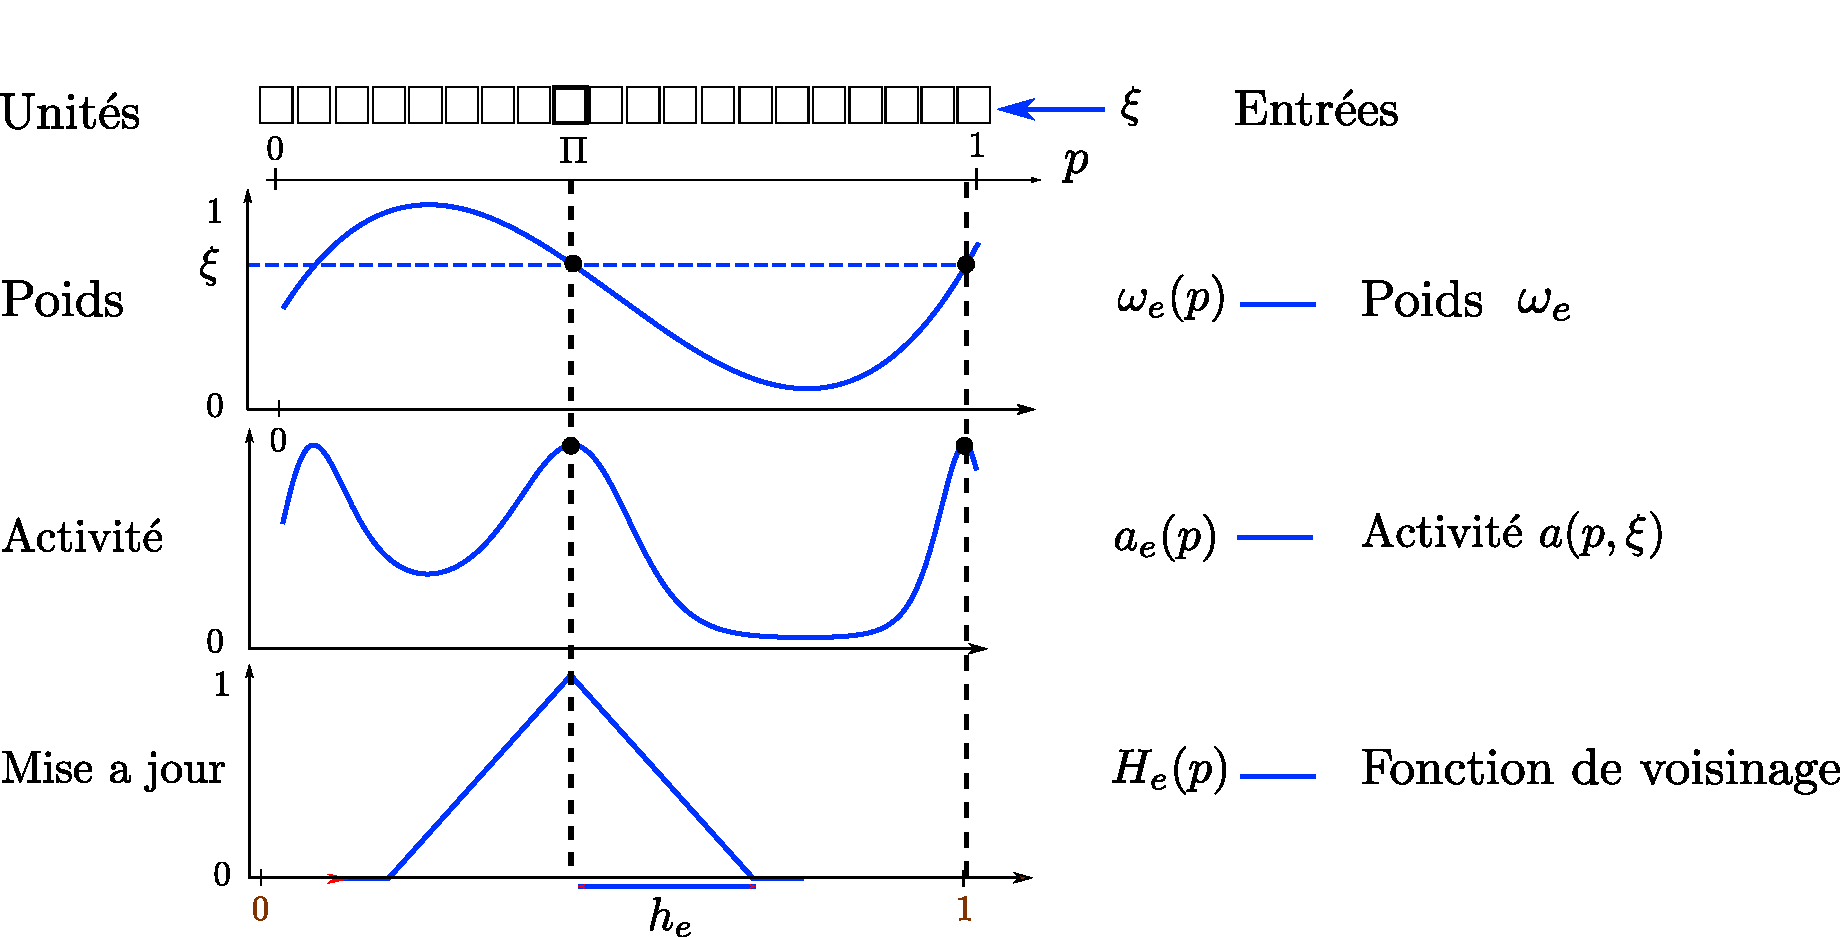
\includegraphics[width=0.6\textwidth]{one_map_one_layer.pdf}
\caption{Notations utilisées dans une carte de Kohonen simple}
\label{fig:one_map_not}
\end{figure}


\subsection{Approche topologique des cartes de Kohonen}

\draft{La notion de voisinage et de topologie est un élément clé des cartes de Kohonen. Le voisinage est en effet pris en compte lors de l'apprentissage et lors de l'interpretation des cartes. Cependant, ce voisinage est généralement défini, dans les applications des cartes, comme un bonus par rapport aux KMeans, une aide à la convergence et à la vitesse de dépliement. Pourtant c'est la l'essence même d'une carte de Kohonen: projeter des éléments sur un graphe, ce qui nous permet de faire des calculs sur des positions plutot que des données de grandes dimensions. 
\begin{figure}
\centering
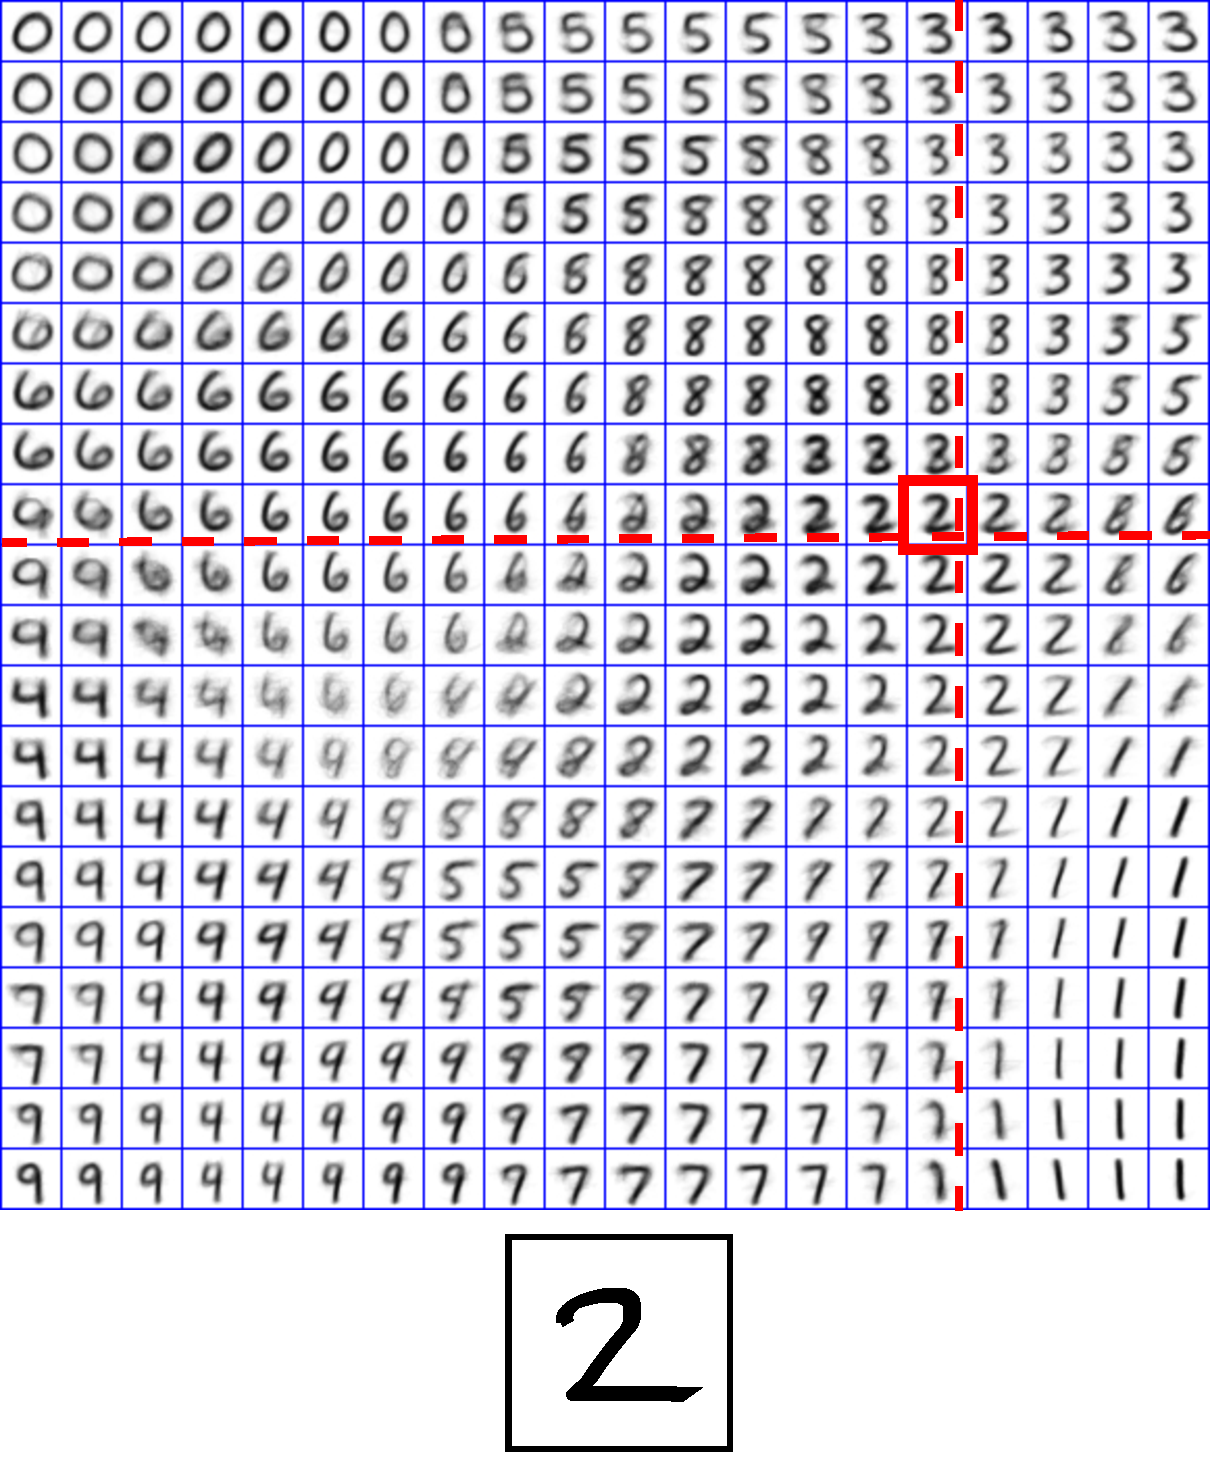
\includegraphics[width=0.3\textwidth]{digits002.pdf}
\caption{Une carte de Kohonen s'organise en zones dont les poids sont proches dans l'espace des entrées. Chaque entrée présentée à la carte peut alors être représentée par la valeur de la position du BMU correspondant dans la carte. Les entrées sont projetées sur le carré $[0,1] \times [0,1]$.}
\end{figure}

}
%\section{Travaux préliminaires sur les architectures de cartes de Kohonen}
\section{Modèle CxSOM}

Le but de cette thèse est de proposer un modèle permettant d'associer des cartes auto-organisatrices dans n'importe quel type d'architecture. En particulier, on cherchera à construire des architectures non-hiérarchiques de cartes, par exemple en figure~\ref{fig:archi_non_hierarchique}.

\begin{figure}
\centering
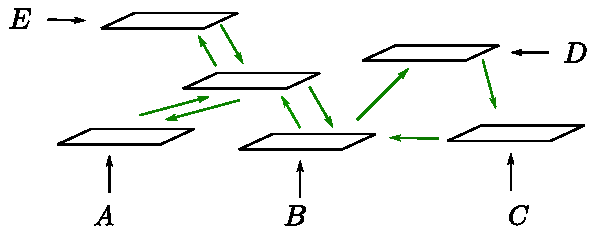
\includegraphics[width=0.6\textwidth]{architecture.pdf}
\caption{Exemple d'architecture modulaire \emph{non-hiérarchique} de cartes de Kohonen. Les entrées sont $A,B,C,D,E$ quelconques. Chaque carte peut ou non prendre une entrée ; les connexions sont réciproques ou non.}
\label{fig:archi_non_hierarchique}
\end{figure}

Dans ce modèle, l'algorithme original de Kohonen est modifié afin de connecter des cartes entre elles, et d'autoriser des connexions non-hiérarchiques.
La connexion entre une carte A et une carte B est réalisée lorsque la carte B prend comme entrée la position du Best Matching Unit de A. 
Considérons G, le graphe de connexions des cartes. Ce graphe est \emph{orienté} et les \emph{boucles} sont autorisées. C'est ce qu'on appelera \emph{architecture non-hiérarchique} de cartes, par opposition à des architectures hiérarchiques dans lesquelles le BMU d'une carte A est donné en entrée d'une carte B de façon unidirectionnelle. 

Chaque carte aura ainsi plusieurs entrées : une entrée \emph{externes} dans un espace d'entrée, facultative, et $k$ entrées \emph{contextuelles} qui sont les positions des BMUs des cartes qui lui sont connectées. Par ailleurs, la recherche du BMU doit être modifiée par rapport à l'originale : les rétroactions entre les cartes sont autorisées, la position du BMU de la carte A va donc influencer la position du BMU de la carte B, lequel modifie à nouveau le BMU de la carte A, etc. 
Notre algorithme implémente donc deux modifications principales par rapport à l'algorithme d'apprentissage d'une carte de Kohonen classique: 
\begin{itemize}
\item Les cartes possèdent plusieurs entrées, externes et contextuelles; les entrées contextuelles sont les positions des BMUs d'autres cartes. Le calcul de l'activité est donc modifié afin de prendre en compte ces différentes couches d'entrées.
\item La recherche du BMU est modifiée afin de gérer les rétroactions entre cartes.
\end{itemize}

La description du modèle CxSOM est détaillée en figure~\ref{fig:one_map}, dans un cas ou une carte reçoit deux connexions, et l'algorithme explicité en~\ref{algo:cxsom}.


\subsection{Gestion des entrées externes et contextuelles}

A un pas d'apprentissage $t$, une carte $M$ reçoit en entrée une entrée \emph{externe} notée $\inpx_t$ et $K$ entrées \emph{contextuelles} notées $\inpc_{0t},\cdots,\inpc_{Kt}$, qui sont les positions des BMU $\bmu$ des cartes qui lui sont connectées. La carte possède donc $k+1$ couches de poids. $\w_e$ correspond à l'entrée externe et $\w_{c0}, \cdots, \w_{cK}$ aux entrées contextuelles. On calcule une activité séparément sur chaque couche de poids selon la formule suivante : 
\begin{equation}
\label{eq:activite}
a(p,x) = \exp(\frac{(\w(p)-x)^2}{2\sigma^2} \; x = \inpx_t\; \text{ou}\; \inpc_{kt}, \; \w = \w_e \;\text{ou}\; \w_{ck}
\end{equation}
Les activités contextuelles sont moyennées en une activité $a_c(p,\mathbf{\inpc}_t)$, avec $\mathbf{\inpc_t} = (\inpc_{0t}, \cdots, \inpc{Kt})$. 
Les activités externes et contextuelles sont enfin fusionnées en une activité globale:
\begin{equation}
\label{eq:global_act}
a_g(p,\inpx_t,\mathbf{\inpc_t}) = \sqrt{a_e(p,\inpx_t)(\beta a_e(p,\inpx_t) + (1-\beta) a_c(p, \mathbf{\inpc_t})}
\end{equation}

Une convolution est appliquée sur cette activité globale. Cela évite les effets de plateau. Seule l'activation globale est considérée lors du calcul du BMU par relaxation, décrit en partie suivante. 

\subsection{Calcul du BMU par relaxation}

Contrairement à une carte simple, on ne peut pas calculer tous les BMUs de l'architecture en prenant l'argmax de $a_g$ dans chaque carte. A cause des influences mutuelles entre cartes, calculer le BMU d'une des cartes modifie les entrées des autres cartes de l'architecture, et donc leur BMU. Cette recherche est donc réalisée par un processus dynamique que l'on appelera \emph{relaxation}, menant à un consensus entre cartes : on cherche le point, s'il existe, où chaque BMU maximise l'activité globale de chaque carte.

Le processus de relaxation est donc une boucle imbriquée dans un pas d'apprentissage de l'architecture, indexée par $\tau$. Notons $\bmu\m[i]$ la position du BMU de la carte $i$, et $\mathbf{\bmu} = (\bmu\m[0], \cdots , \bmu\m[n])$, avec $n$ le nombre de cartes de l'architecture.
Au début d'un pas d'apprentissage, chaque carte est nourrie avec une entrée externe $\inpx^i_t$, et les activités externes $a_e^i(\inpx^i_t,p)$ de chaque carte peuvent être calculées.
La recherche du BMU suit le processus de relaxation suivant : 
\begin{enumerate}
\item Dans chaque carte $i$, la position $\bmu^i$ est initialisée à $\argmax_p(a_e^i(\inpx^i_t,p)$. Les entrées contextuelles sont alors initialisées en prenant le BMU correspondant aux connexions de l'architecture.
\item Tant que toutes les positions $\bmu^i$ ne sont pas stables, 
	\begin{enumerate}
	\item Dans chaque carte $i$, calculer les activités contextuelles et globales, définissant ainsi $p^{\star i} = \argmax_p(a_g(p,\mathbf{\inpc^i},\inpx^i)$
	\item Déplacer $\bmu^i$ vers $p^{\star i}$ : $\bmu^i \leftarrow \bmu^i \pm \Delta$ si $\lvert \bmu^i - p^{\star i} \rvert \geq \Delta$, $\bmu^i \leftarrow p^{\star i}$ sinon
	\end{enumerate}
	
\item Le BMU de chaque carte est pris comme la valeur finale stable de ce processus dynamique. Cette valeur est utilisée pour les mise a jour des poids.
\end{enumerate}

Il peut arriver que les positions se stabilisent sur un cycle limite. Dans ce cas, on arrêtera la relaxation arbitrairement; ce phénomène étant ponctuel, il n'influence pas l'apprentissage. Les paramètres des cartes de l'architecture sont choisis pour éviter de telles situations.

\begin{figure}
\centering
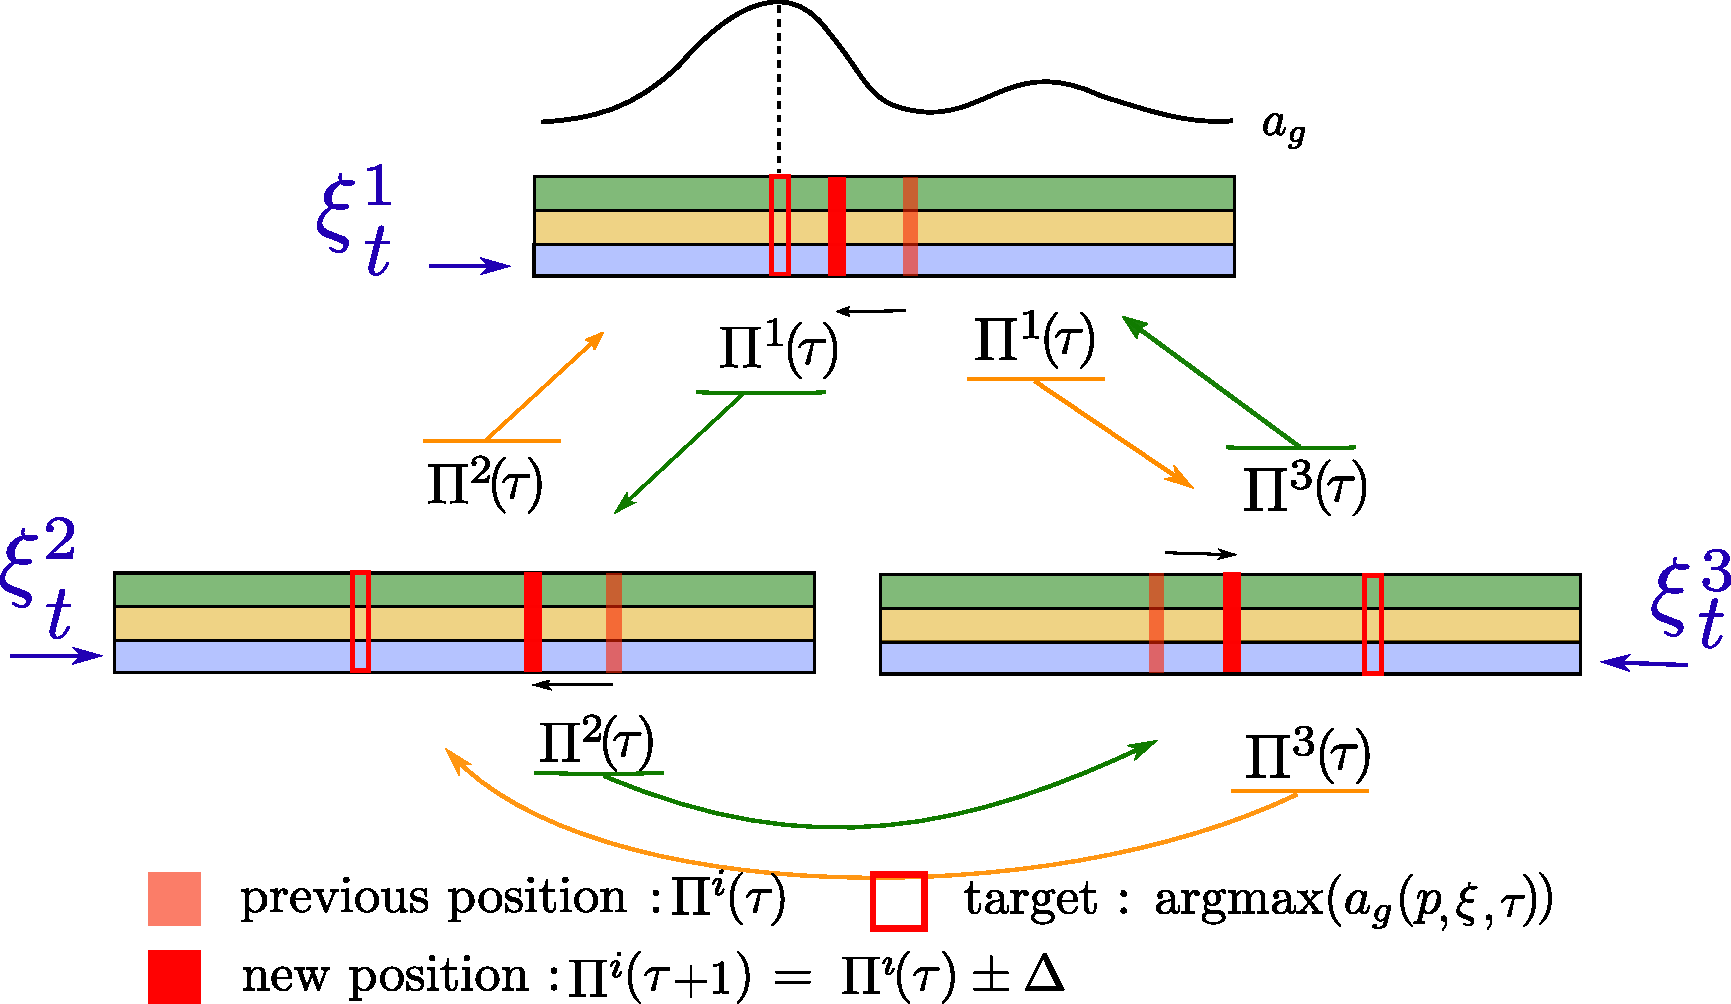
\includegraphics[width=0.6\textwidth]{relaxation.pdf}
\label{fig:relax}
\caption{description d'une étape de la relaxation dans l'architecture, aboutissant à un consensus entre cartes. Au sein d'une même itération $t$, les position des BMU $\bmu$ sont légèrement déplacées jusqu'à ce que toutes les positions $\bmu$ des cartes de l'architecture soient stable. Ces positions maximisent collectivement les activités globales de chaque carte. }
\end{figure}

\begin{figure}
\centering
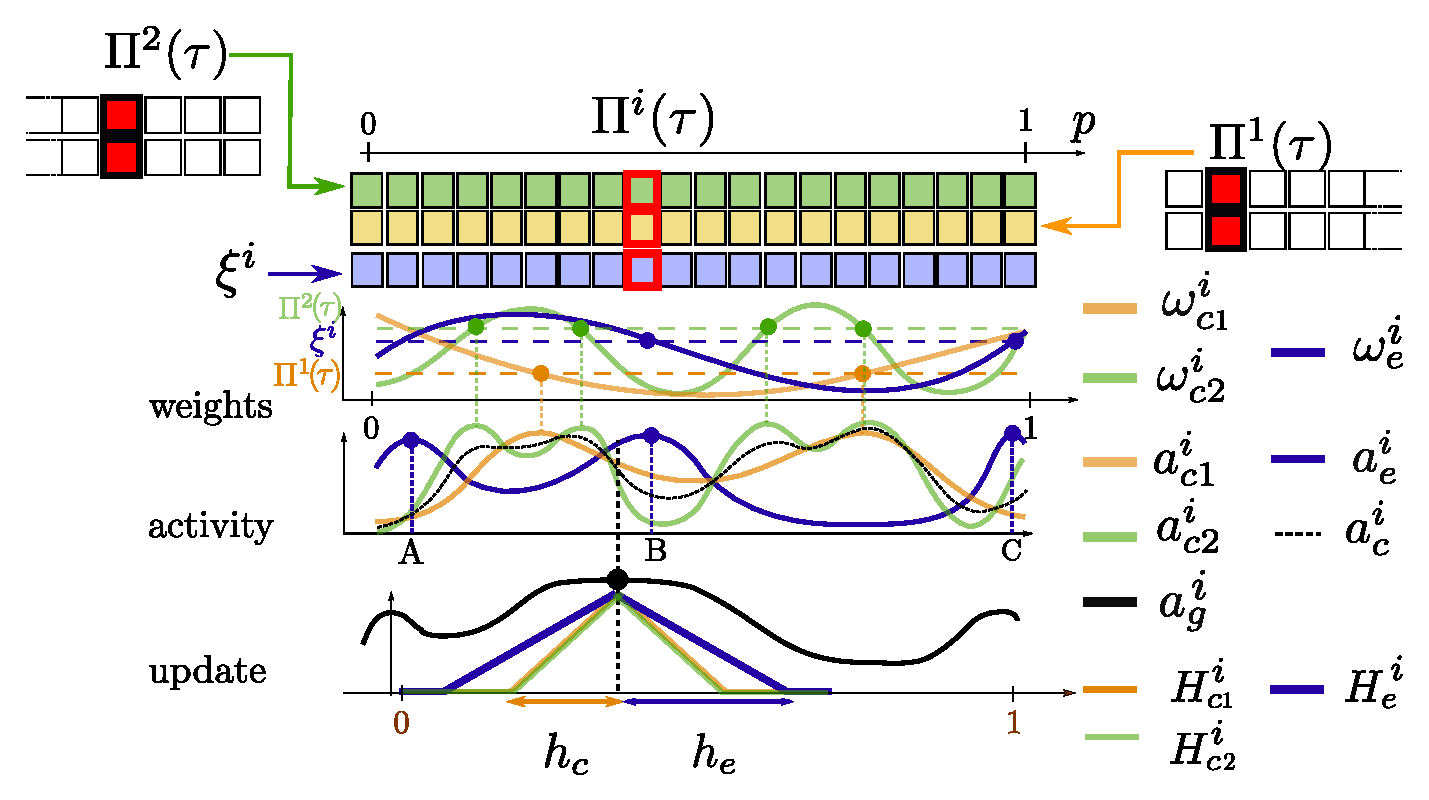
\includegraphics[width=0.8\textwidth]{one_map.pdf}
\caption{Description d'une carte au sein d'une architecture CxSOM. La carte recoit deux connexions de cartes voisines, et possède donc deux couches contextuelles}
\label{fig:one_map}
\end{figure}

\subsection{Mise à jour des poids}

Les poids sont mis à jour par rapport à leurs entrées respectives suivant l'équation \ref{eq:update}. Le BMU d'une carte est ainsi commun à toutes les couches. Les rayons de voisinage $h_e$ et $h_c$ ont des valeurs différentes ; celles-ci seront détaillée en partie suivante. 

\subsection{Résumé : Algorithme général}





